\documentclass[9pt,t]{beamer}
% note that full page width is 12.8 cm and height is 9.6 cm

\mode<presentation>
{
  \usepackage[headline,footline]{beamerthemelectures}

}

% load packages
\usepackage[english]{babel}
\usepackage{graphicx}
\usepackage{multimedia}
%\usepackage[T1]{fontenc}
\usepackage{lmodern}
\usepackage{amsmath,amssymb}
\usepackage{pgf,booktabs,verbatim}
\usepackage{pgfarrows,pgfnodes}
\usepackage[absolute,overlay]{textpos}
\setlength{\TPHorizModule}{\paperwidth}
\setlength{\TPVertModule}{\paperheight}
\usepackage{tikz}

\setbeamertemplate{frametitle}{
\begin{centering}
\insertframetitle
\par
\end{centering}
} 

% create command to add nice looking citation
\newcommand{\reference}[1]{\flushright \vspace{-0.3cm} {\tiny #1}} 


\title{Solutions to Modeling Exercise \#4\\ Thermohaline circulation}

\begin{document}

\section{}

%%%
\frame{
    \frametitle{\vspace{1cm}\huge Thermohaline circulation}
    Note: The terms ``hot'' and ``cold'' refer to the state of the Arctic/Antarctic.   
}

\frame{
\frametitle{1. Evolution to steady state}
\begin{figure}
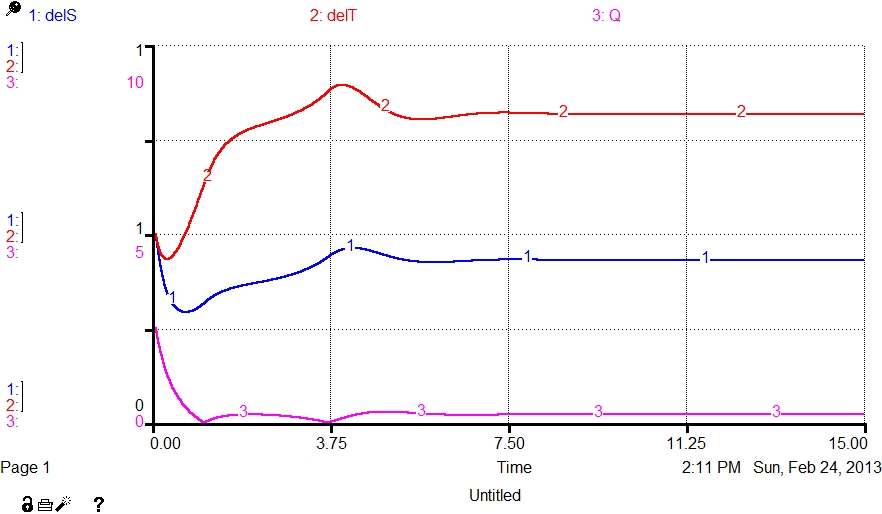
\includegraphics[width=0.9\textwidth]{./p1a.jpg}
\end{figure}
\begin{itemize}
\item Initial run to ``cold and slow'' steady state
\item Large temperature difference balanced by large salinity difference $\Rightarrow$ low flux (cold water wants to sink, but freshwater doesn't want to sink)
\end{itemize}
}

\frame{
\frametitle{1. Evolution to steady state}
\begin{figure}
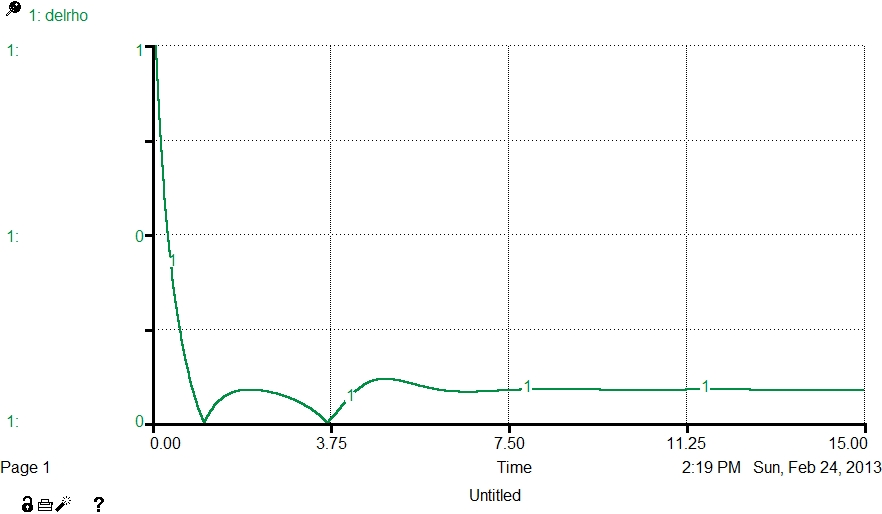
\includegraphics[width=0.9\textwidth]{./p1b.jpg}
\end{figure}
\begin{itemize}
\item Small density difference in ``cold and slow'' state
\end{itemize}
}

\frame{
\frametitle{2. Multiple steady-states}
\begin{figure}
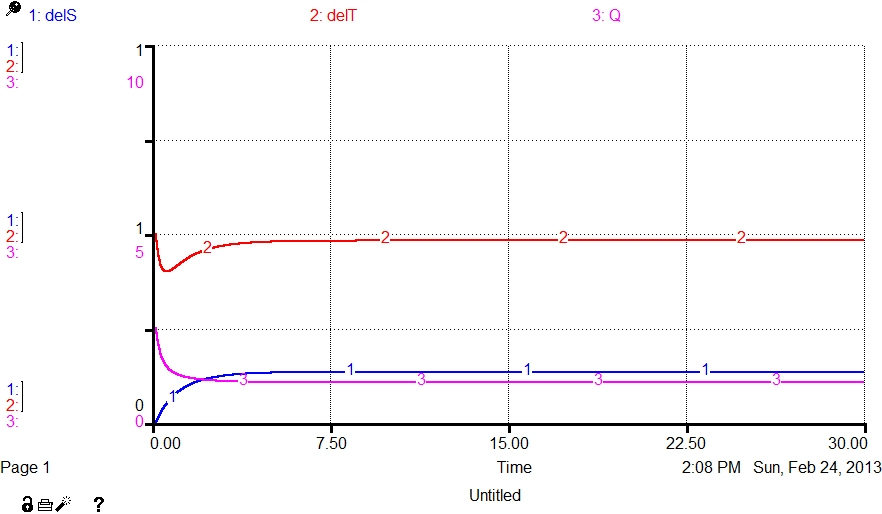
\includegraphics[width=0.9\textwidth]{./p2a.jpg}
\end{figure}
\begin{itemize}
\item Run to ``warm and fast'' steady state
\item Temperature difference is much larger than the salinity difference\ldots
\end{itemize}
}

\frame{
\frametitle{2. Multiple steady-states}
\begin{figure}
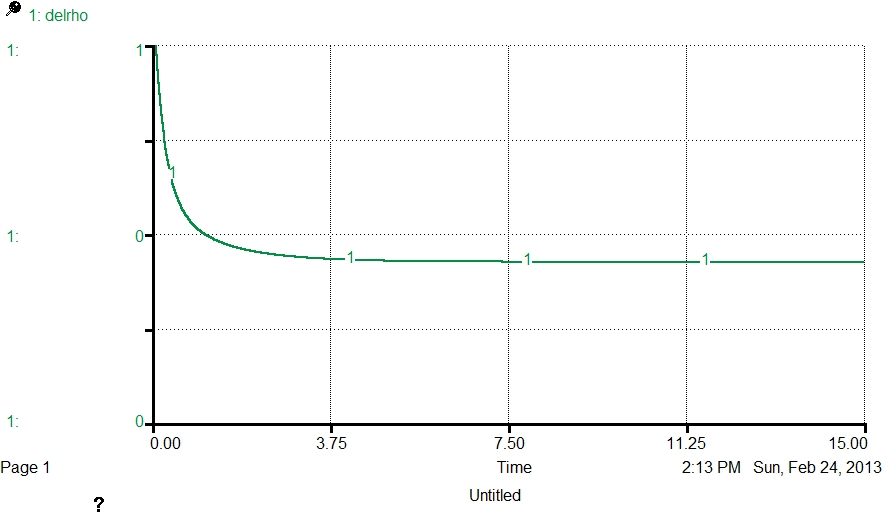
\includegraphics[width=0.9\textwidth]{./p2b.jpg}
\end{figure}
\begin{itemize}
\item \ldots leading to a large density difference
\end{itemize}
}

\frame{
\frametitle{2. Multiple steady-states}
\begin{figure}
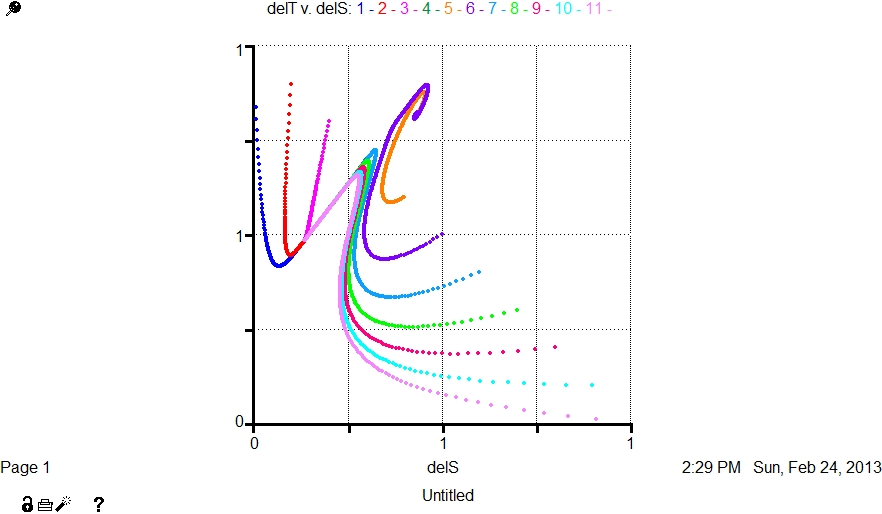
\includegraphics[width=0.9\textwidth]{./p2c.jpg}
\end{figure}
\begin{itemize}
\item Model has two possible steady states
\begin{itemize}
\item Cold and slow state (0.45, 0.8)
\item Warm and fast state (0.125, 0.5)
\end{itemize}
\end{itemize}
}

\frame{
\frametitle{3. Warming climate}
\begin{figure}
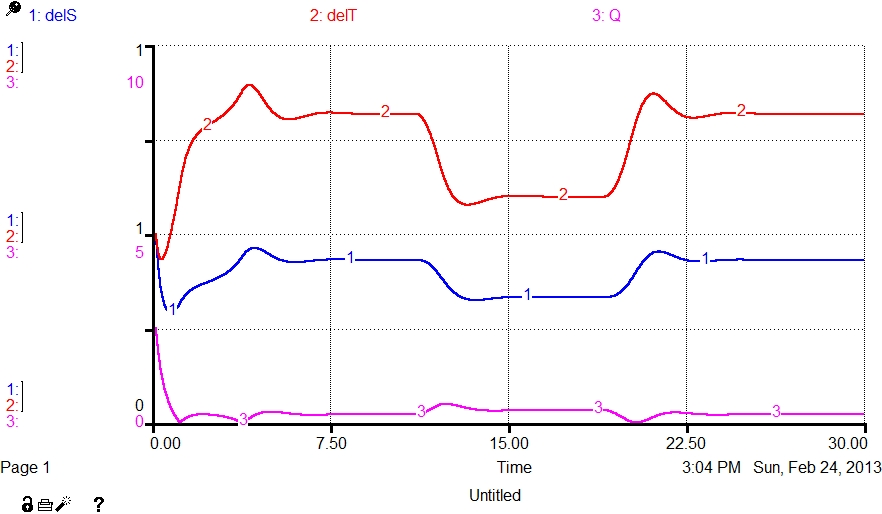
\includegraphics[width=0.9\textwidth]{./p3a.jpg}
\end{figure}
\begin{itemize}
\item From the cold state, temporarily decrease the temperature gradient to 0.6
\item Returns to the cold state
\end{itemize}
}

\frame{
\frametitle{3. Warming climate}
\begin{figure}
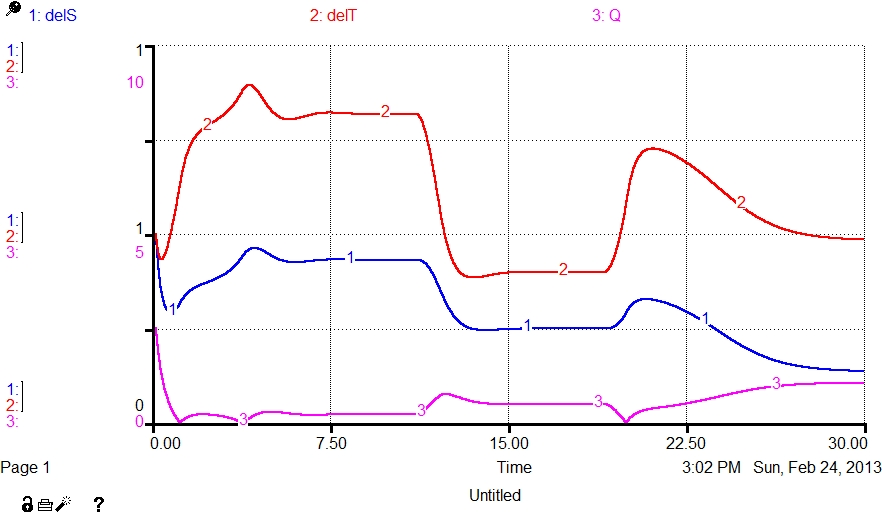
\includegraphics[width=0.9\textwidth]{./p3b.jpg}
\end{figure}
\begin{itemize}
\item From the cold state, temporarily decrease the temperature gradient but using a smaller temperature gradient of 0.4
\item Switches to the warm state
\end{itemize}
}

\frame{
\frametitle{3. Warming climate}
\begin{figure}
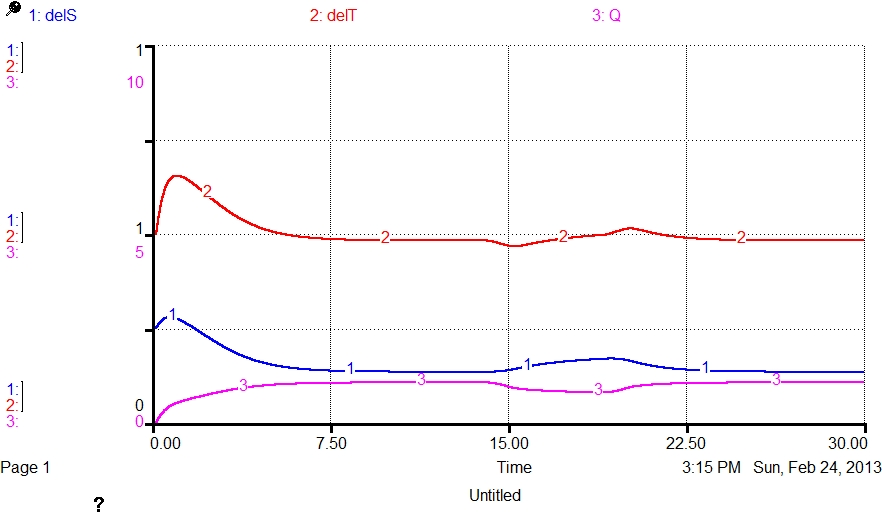
\includegraphics[width=0.9\textwidth]{./p3c.jpg}
\end{figure}
\begin{itemize}
\item From the warm state, temporarily decrease the temperature gradient $\rightarrow$ returns to initial state
\end{itemize}
}

\frame{
\frametitle{3. Warming climate}
\begin{figure}
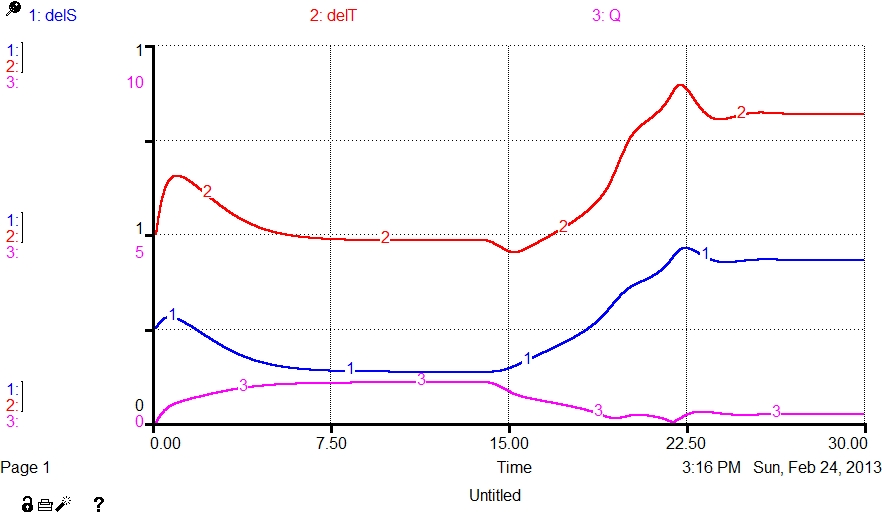
\includegraphics[width=0.9\textwidth]{./p3d.jpg}
\end{figure}
\begin{itemize}
\item From the warm state, temporarily decrease the temperature gradient a little bit more $\rightarrow$ switches to the cold state
\end{itemize}
}

\frame{
\frametitle{3. Warming climate}
\begin{figure}
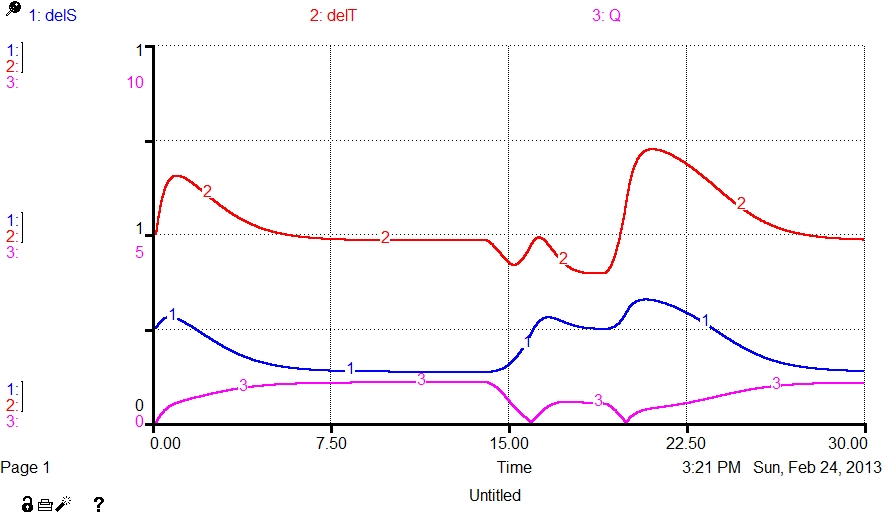
\includegraphics[width=0.9\textwidth]{./p3e.jpg}
\end{figure}
\begin{itemize}
\item From the warm state, temporarily decrease the temperature gradient even a little bit more $\rightarrow$ returns to the initial state
\end{itemize}
}

\frame{
\frametitle{4. Freshwater pulses}
\begin{figure}
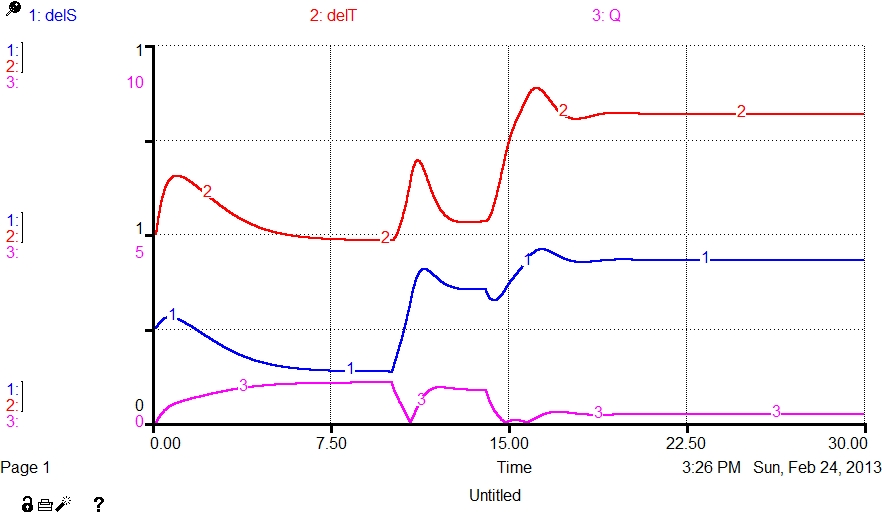
\includegraphics[width=0.9\textwidth]{./p4a.jpg}
\end{figure}
\begin{itemize}
\item From the warm state, increase the salinity difference
\end{itemize}
}

\frame{
\frametitle{4. Freshwater pulses}
\begin{figure}
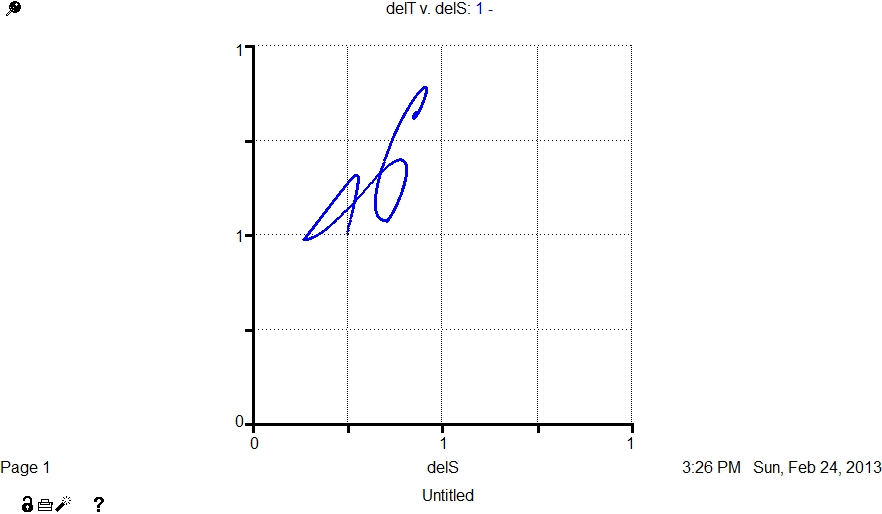
\includegraphics[width=0.9\textwidth]{./p4b.jpg}
\end{figure}
\begin{itemize}
\item Transitions from the ``warm and fast'' state to the ``cold and slow'' state
\end{itemize}
}

\frame{
\frametitle{Key ideas}
\begin{itemize}
\item System parameters can vary unpredictably as a system evolves toward a steady-state
\item The initial conditions matter $\rightarrow$ systems often have multiple steady states; the initial conditions determine which steady state a system will approach
\item Short pertubations can cause a ``permanent'' transition from one state to another
\item Observed a transition out of the (i) cold state for large perturbations in temperature (ii) warm state for moderate perturbations in temperature
\item Also produced transitions from one state to another by modifying the salinity difference
\end{itemize}
}

\end{document}
